

\section{「滞在ウォッチ」のシステム構成}\label{3.1}
% 本研究のシステム概要を図\ref{StayWatchOverview}に示す.
滞在ウォッチは,ビーコンを持ち歩き在室情報を記録するメンバ,メンバ管理,メンバへのビーコン配布,利用者の登録を行う管理者,現在状況や履歴を閲覧したりAPIを通して在室情報を利用する利用者(メンバや管理者も利用者になりうる),システムを開発する開発者がおり,メンバがビーコンを携帯し,部屋ごとに設置された受信機によりビーコンを検出する手法で,在室者管理を自動に行う.
本研究のシステム概要を図\ref{StayWatchOverview}に示す.
メンバには一人1つビーコンを携帯してもらう.サーバには部屋メンバの名前とビーコンのIDを登録する.ビーコンは周囲に数秒に1回電波を発信する.
% 受信機がビーコンの電波を受信する間隔は3分である.
受信機が検出したビーコンのIDと電波強度は日時や在室した部屋名とともにサーバに送信され記録される.
記録した在室者情報はWeb APIを通して利用可能であり,勤怠管理システムや来訪促進システムといった様々な応用を想定している.

\begin{figure}[h]
  \centering  % 図を真ん中に配置
  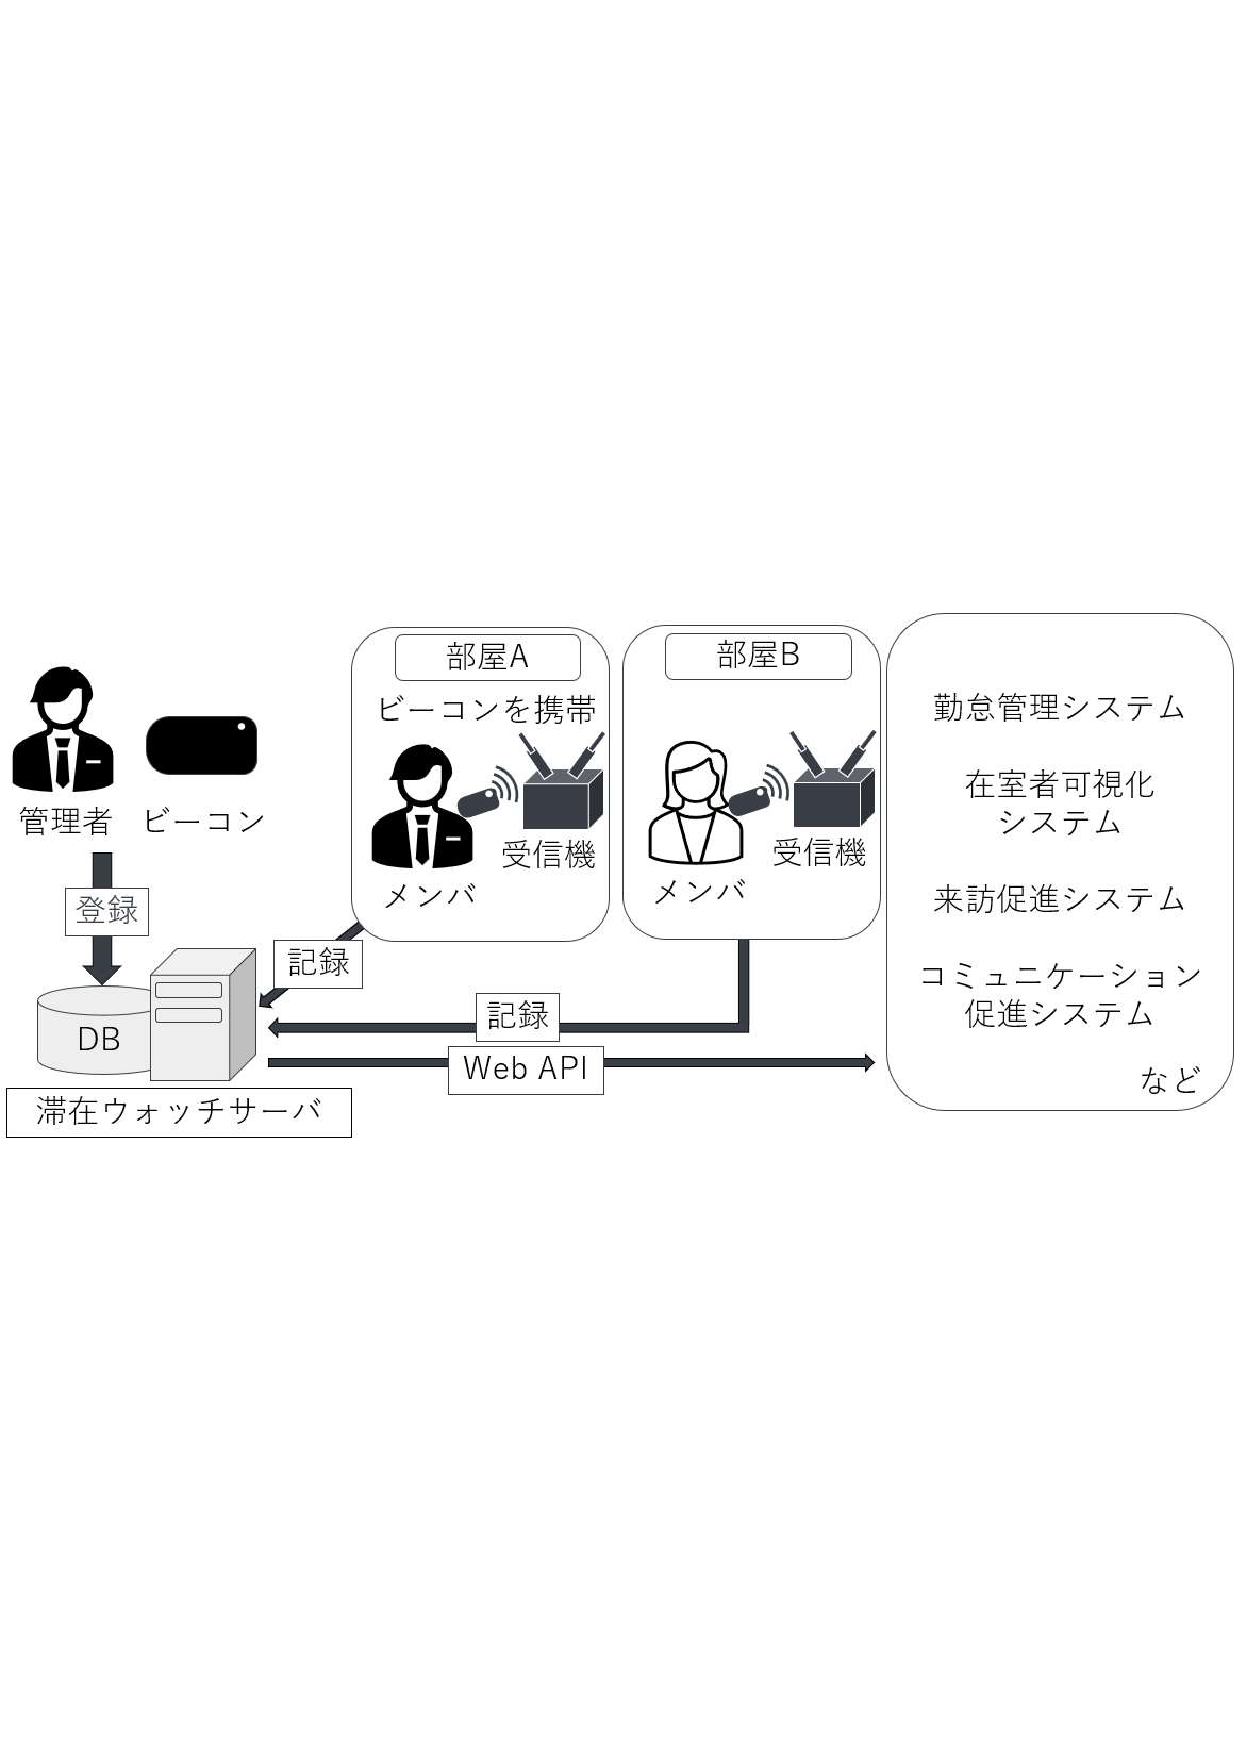
\includegraphics[clip,scale = 0.6]{image/system.pdf}
  \caption{「滞在ウォッチ」の概要図}    \label{StayWatchOverview}
\end{figure}

本手法に関連するビーコン,受信機,サーバを示す.
メンバが携帯するビーコンには,長期的な運用を考慮しバッテリ交換が可能かつ小型なFCS1301\cite{fcs1301}を利用している.
ビーコンは図\ref{fig:beacons}のように様々な大きさや形のものがある.
複数のビーコンの比較を表\ref{tb:beacons}に示す.
ボタンは定期的な電波発信に加えて押した時にも電波発信できるため,点検時に利用できる.
FCS1301の用途は,財布やパスケースなどの貴重品に付ける紛失防止や子供の荷物などに付ける見守り支援がある.
% 実際にパスケースに取り付けた様子を図\ref{fig:beaconforpass}に示す.
財布やパスケースに取り付けたり入れられるサイズである.
そのため,メンバが携帯するのに適している.
またバッテリ交換の際の様子を図\ref{fig:batchange}に示す.
特殊な器具などを使う必要がなく,簡単にバッテリ交換ができる.
FCS1301ではボタンを押すとペアリング,長押しするとスリープモードへ移行し,保管の間省電力モードになる.
ビーコンの電波送信の間隔はFCS1301の規格で最大の10秒ごとに設定している.
1部屋ごとに台設置する受信機には図\ref{fig:raspi} の低価格な Raspberry Pi\cite{raspi} を利用している.
1つの部屋に1つずつ受信機を設置する.
% サーバには,Google Cloud Platform\cite{gcp}を利用している.

\begin{figure}[H]
  \begin{center}
    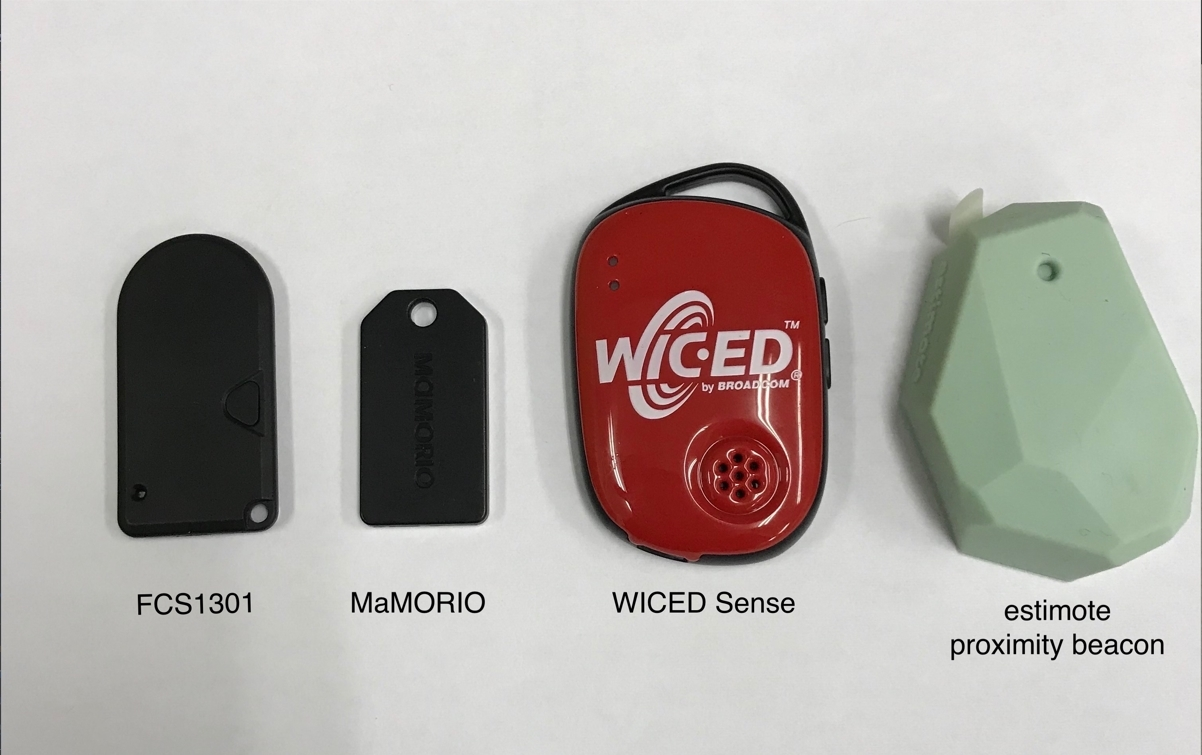
\includegraphics[width=150mm]{image/beaconType.jpg}
    \caption{ビーコンの種類}
    \label{fig:beacons}
  \end{center}
\end{figure}

\begin{table}[H]
  \begin{center}
    \caption{ビーコンの比較}
    \label{tb:beacons}
    \begin{tabular}{|l|c|c|c|} \hline
      ビーコン名    & サイズ                           & バッテリ交換 & ボタン \\ \hline \hline
      FCS1301  & 縦46.0 mm× 横24.5 mm× 厚さ3.5 mm  & ○      & ○   \\
      MAMORIO  & 縦35.5 mm× 横19.0 mm× 厚さ3.4 mm  & ×      & ×   \\
      WICED    & 縦60.0 mm× 横37.0 mm× 厚さ10.0 mm & ○      & ○   \\
      estimote & 縦55.0 mm× 横38.0 mm× 厚さ15.0 mm & ×      & ×   \\\hline
    \end{tabular}
  \end{center}
\end{table}

% \begin{figure}[H]
%   \begin{center}
%     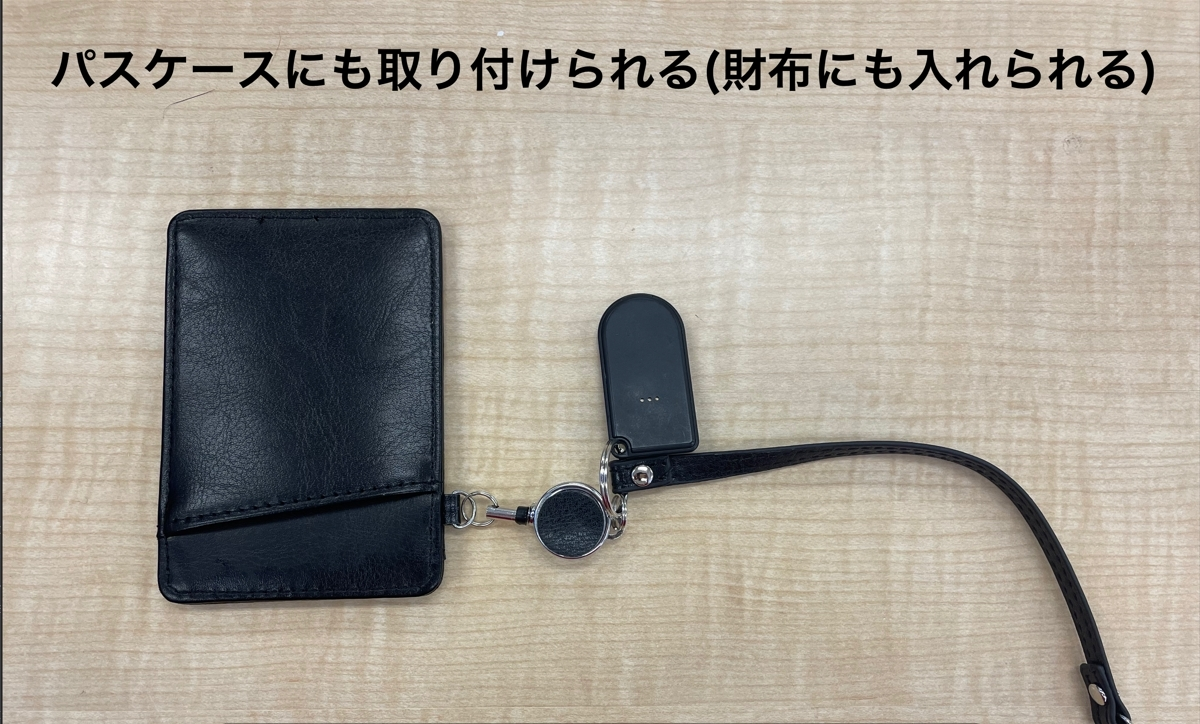
\includegraphics[width=150mm]{image/beaconForpass.jpg}
%     \caption{パスケースに取り付けたビーコン}
%     \label{fig:beaconforpass}
%   \end{center}
% \end{figure}

\begin{figure}[H]
  \begin{center}
    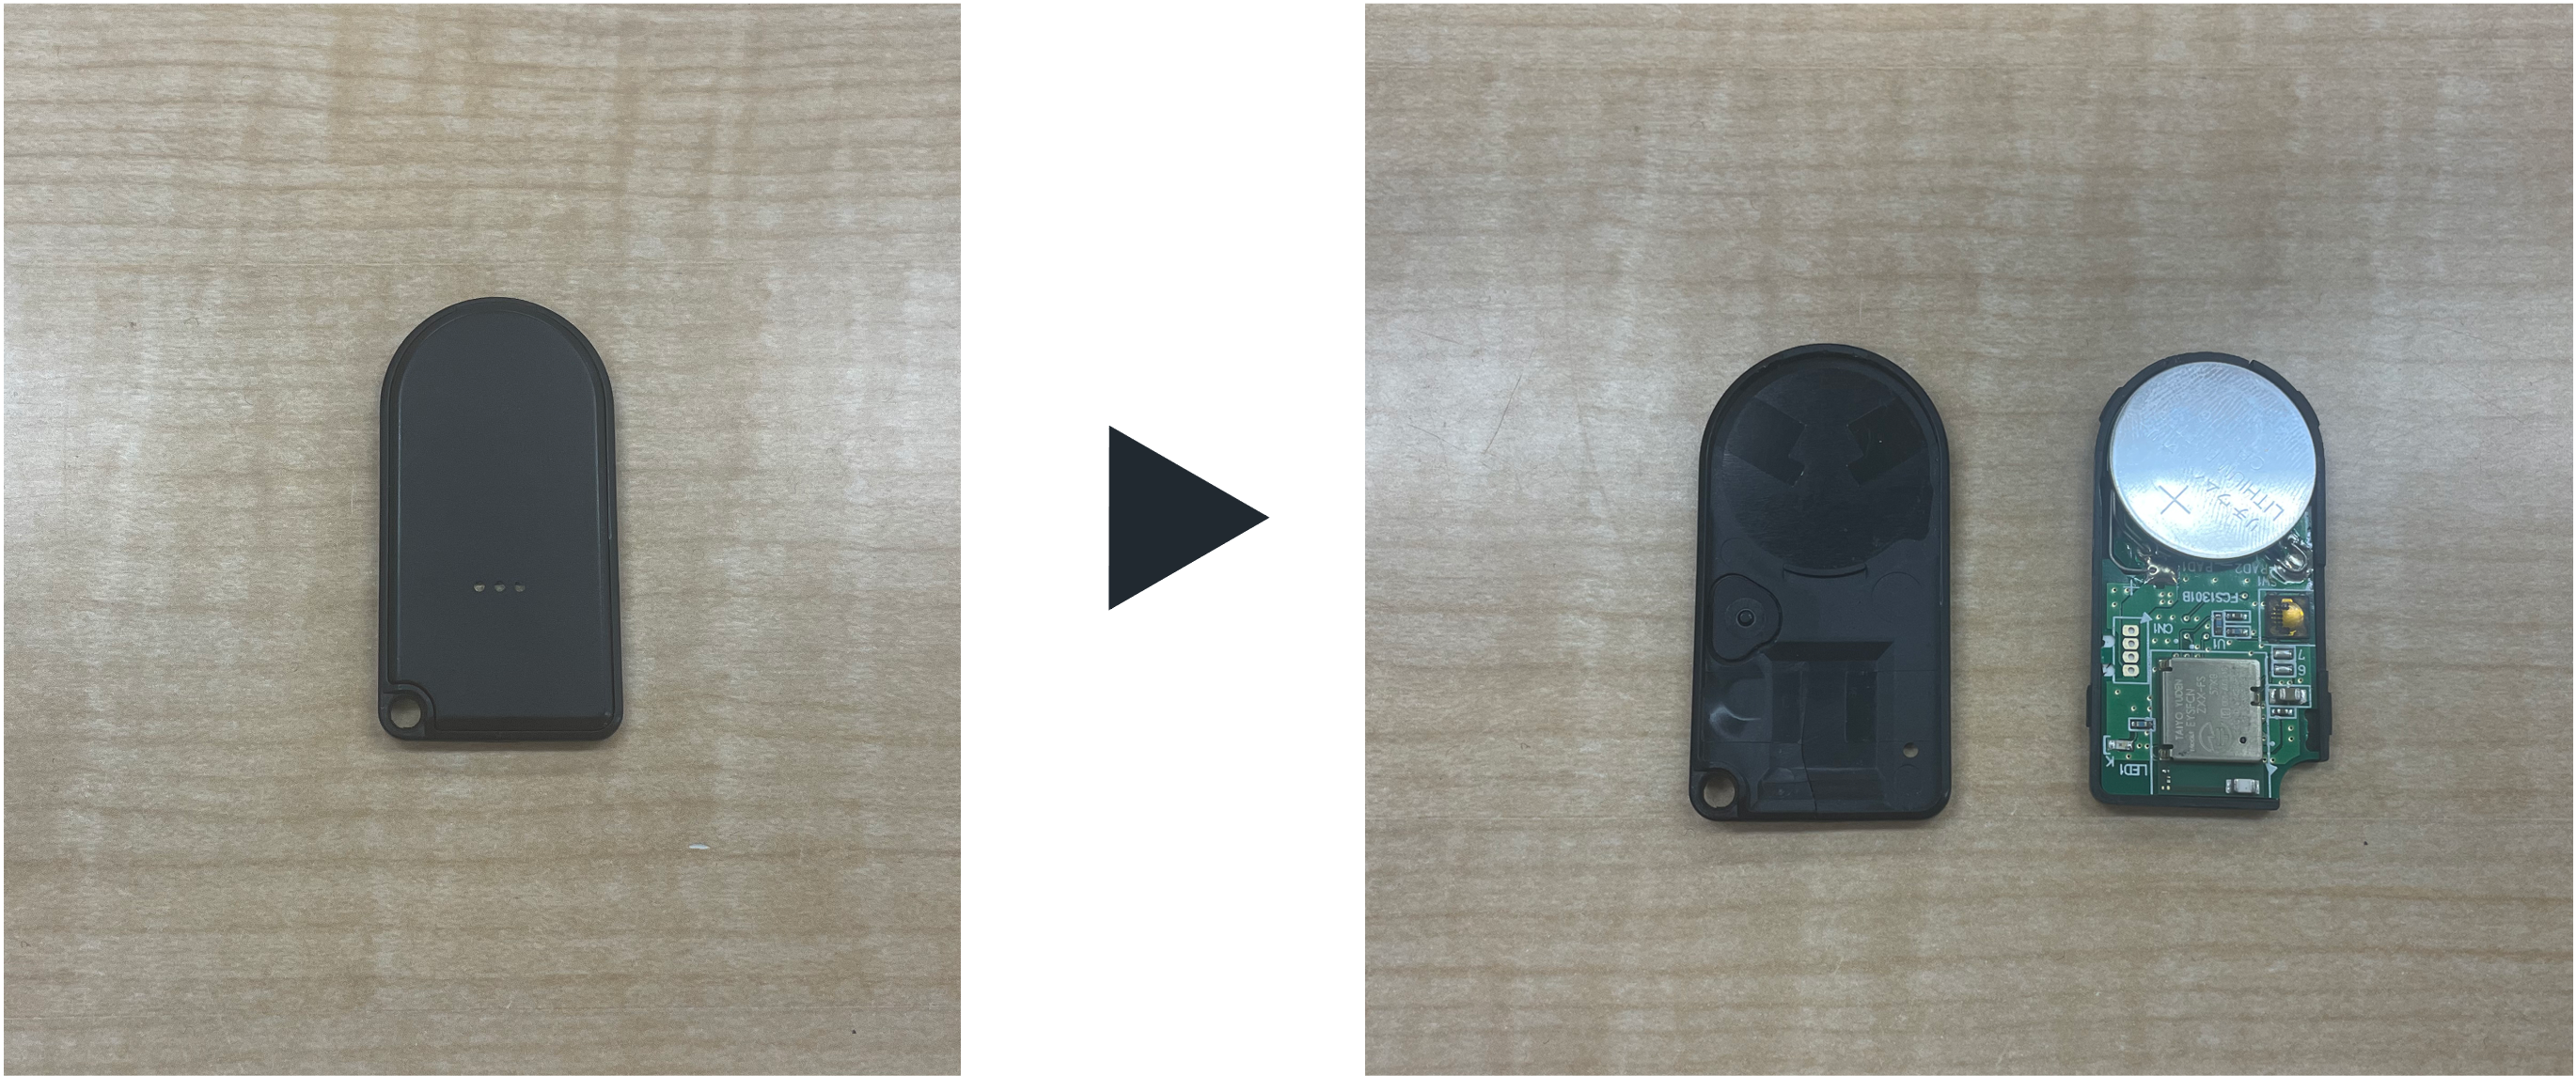
\includegraphics[width=150mm]{image/batchange.png}
    \caption{ビーコンのバッテリ交換}
    \label{fig:batchange}
  \end{center}
\end{figure}

\begin{figure}[H]
  \begin{center}
    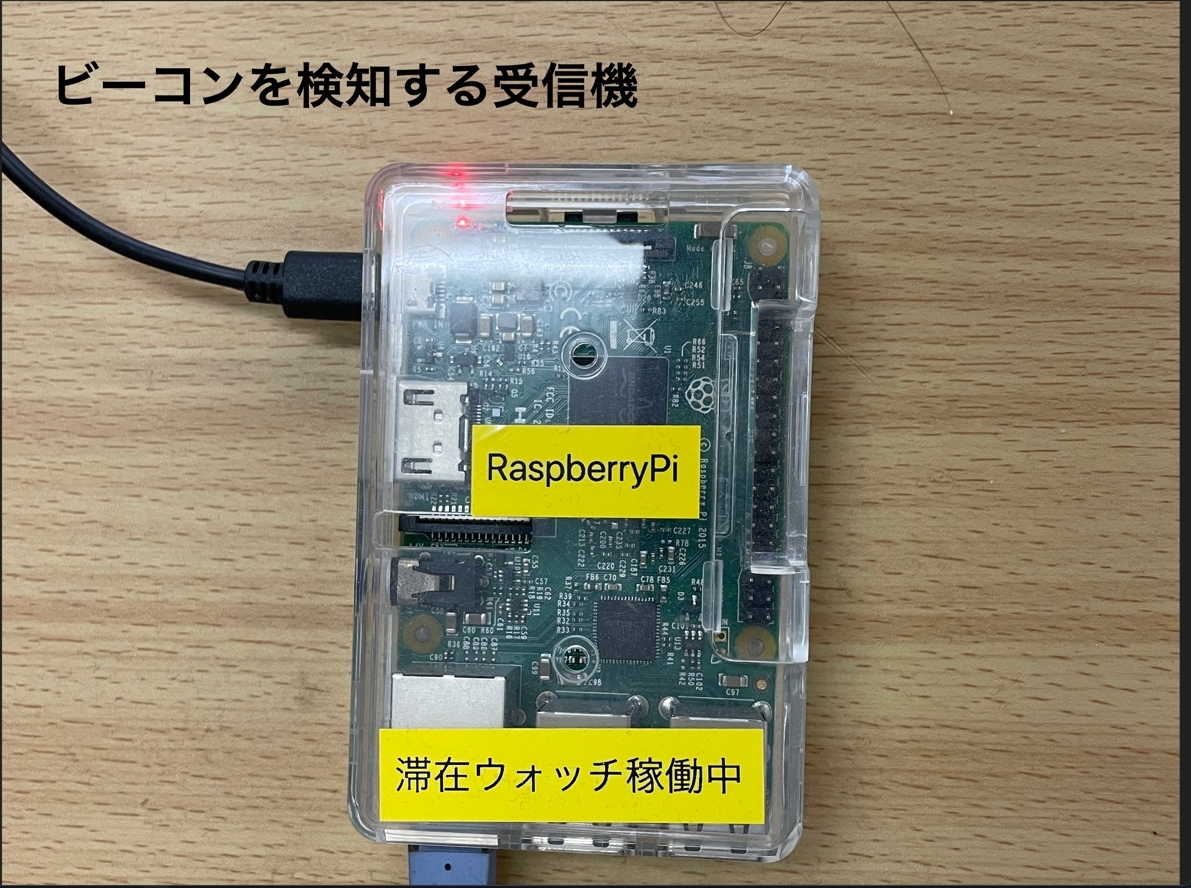
\includegraphics[width=150mm]{image/RasPi.jpg}
    \caption{実際に使用しているビーコンを検知する受信機}
    \label{fig:raspi}
  \end{center}
\end{figure}

% 個人を特定する在室者の検出手法には,個人と在室者情報を紐付けする必要がある.
% ビーコンを用いた検出手法ではビーコンのIDとメンバの名前をサーバのデータベースに登録している.
% 登録には図\ref{fig:ent}のウェブサイトを用いて行う.
% グループ分けとして研究室やチームの属性を追加している.
% これは可視化において個人の識別を容易にし,来訪促進システムでは連帯感や競争心を刺激でき,ゲーミフィケーション\cite{gamification}を取り入れる上で有用な情報だと考えている.
% UUID,major,minorはビーコン固有の識別子であり,先述のビーコンのIDに該当する.

% \begin{figure}[H]
%   \begin{center}
%     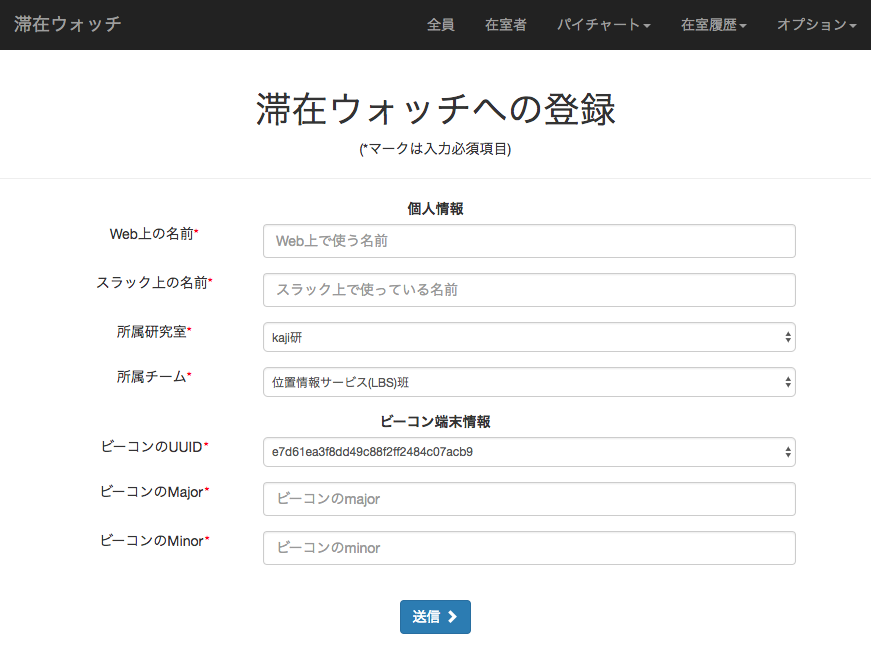
\includegraphics[width=160mm]{image/RegistrationScreen.png}
%     \caption{登録画面}
%     \label{fig:ent}
%   \end{center}
% \end{figure}

メンバがビーコンを携帯し部屋に訪れると,部屋ごとに設置された受信機でビーコンを検出する.
受信機が送信するデータをJSON形式で図\ref{fig:rasPost4}に示す.
Beaconsの配列にはUUIDとRSSIのキーとプロパティを持つオブジェクトが格納されている.
UUIDはビーコンに割り当てられた固有のIDであり,RSSIはビーコンからの受信信号強度である.
RSSIの値はDBM(デシベル・ミリワット)で表される.信号強度が高いほどRSSIの値は大きくなり,信号強度が低いほどRSSIの値は小さくなる.通常-30dBmから-90dBmの範囲で表され-30dBMから-50dBmの範囲は強い信号とされており,-70dBmから-90dBmの範囲は弱い信号とされている.
このデータではUUIDとRSSIのデータを持つオブジェクトが4つ存在しているためメンバのビーコンが4つ検出されている.
さらにBEACONSとROOMIDをラップしたオブジェクトを作成している.ROOMIDは各部屋の受信機ごとに割り当てられた固有のIDであり.ENVファイルに記述されている環境変数である.
受信機側のプログラムはPythonで実装されており,Pythonで受信したデータと.ENVファイルから読み込んだROOMIDを利用して辞書型で図\ref{fig:rasPost4}のような形式のデータを作り
JSON形式に変換してPOSTメソッドでサーバに送信する.


\begin{figure}[H]
  \begin{center}
    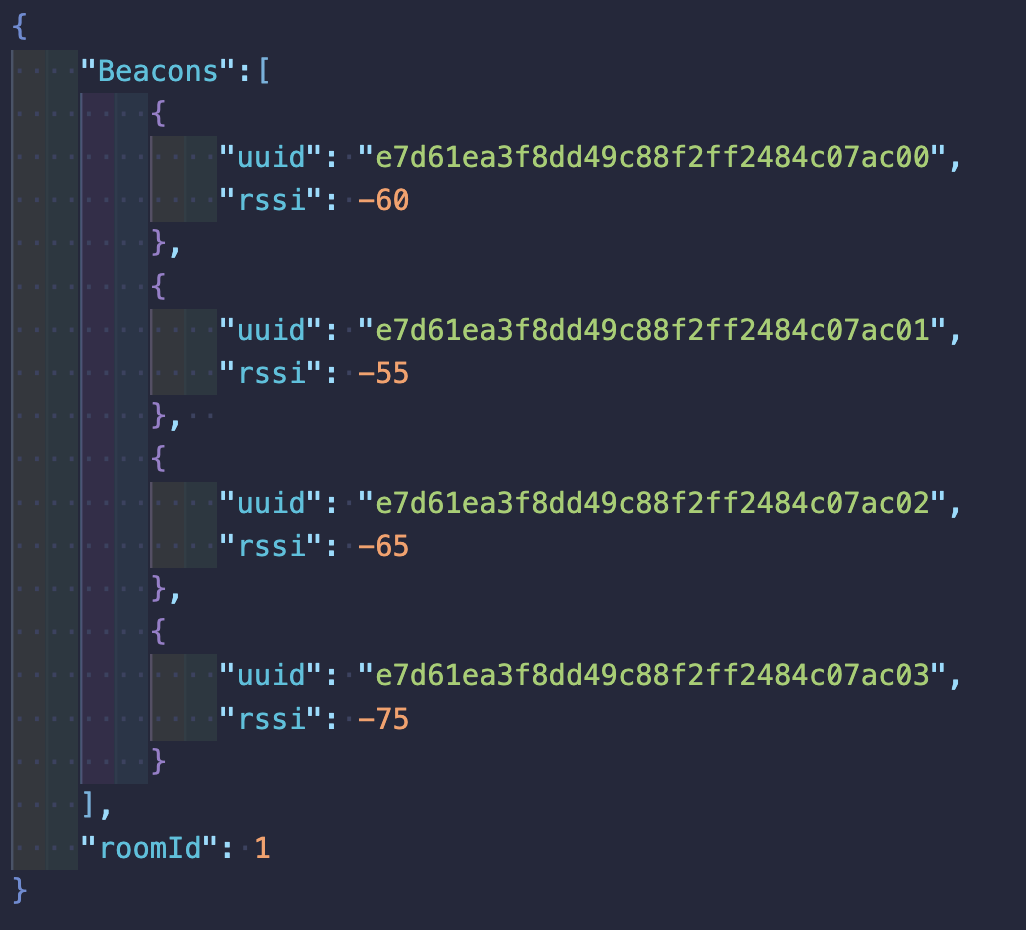
\includegraphics[width=160mm]{image/rasPost4.png}
    \caption{4人分のビーコン情報をサーバに送信する際のデータ}
    \label{fig:rasPost4}
  \end{center}
\end{figure}

受信機から送られてきたデータをサーバ側で処理する.
データベースには現在在室している人の情報の保存を行うStayersテーブルが存在する.
サーバ側のプログラムはStayerテーブルと受信機側から送信されたデータを比較して,Stayersテーブルの情報を更新する.Stayerテーブルのカラムが存在しない場合に図\ref{fig:rasPost4}の形式のデータを受信した場合,受信したROOMIDとUUIDを後述する表\ref{table:users}に示すUsersテーブルと表\ref{table:rooms}に示すRoomsテーブルを参照してStayersテーブルに新しい4つのレコードを追加する.この状態で図\ref{fig:rasPost0}に示すビーコン情報が存在しないデータを受信した場合,その部屋には誰も存在しておらず在室者は退出したと判断しStayersテーブルからレコードを削除する.

部屋ごとに受信機を設置する際に,設置する部屋が隣接する場合にビーコンは周囲数メートルから数十メートルに電波を発信するため,隣接した複数の部屋で同様の在室判定を行う可能性がある.
そこで,ビーコンが発信する電波強度に着目する.
ビーコンの電波強度は表\ref{tb:rf}に示すように壁や扉のコンクリートや鉄板の障害物によって減衰する\cite{barrier}.
そのため,隣接した複数の部屋では電波強度に明らかな差があると考えられる.
受信機から送られてきた電波強度を比較すれば,正確な在室判定が可能である.
したがって,在室判定にビーコンの受信電波強度を利用して隣接した部屋での誤検出の防止が可能だと考える.
% この具体的な例として図\ref{fig:rasPost4}の隣接したROOMIDが別の部屋のIDである場合を挙げる.
% このパターンの場合Stayersテーブルに存在しているRSSIの値よりRSSIの信号強度が高い場合,部屋を移動したと判断しStayersテーブルのROOMIDとRSSIの値を更新する.

\begin{table}[]
  \caption{Stayersテーブル}
  \centering
  \scalebox{1.2}{
    \begin{tabular}{|l|l|l|}
      \hline
      プロパティ      & 型        & 説明               \\ \hline
      id         & bigint   & 主キー              \\ \hline
      user\_id   & bigint   & 副キー(ユーザテーブルの主キー) \\ \hline
      room\_id   & bigint   & 副キー(ルームテーブルの主キー) \\ \hline
      rssi       & bigint   & 電波強度             \\ \hline
      create\_at & datetime & 作成日時             \\ \hline
      update\_at & datetime & 更新日時             \\ \hline
      delete\_at & datetime & 削除日時             \\ \hline
    \end{tabular}
  }\label{table:stayers}
\end{table}


\begin{table}[]
  \caption{Roomsテーブル}
  \centering
  \scalebox{1.2}{
    \begin{tabular}{|l|l|l|}
      \hline
      プロパティ      & 型        & 説明   \\ \hline
      id         & bigint   & 主キー  \\ \hline
      name       & longtext & 部屋名  \\ \hline
      create\_at & datetime & 作成日時 \\ \hline
      update\_at & datetime & 更新日時 \\ \hline
      delete\_at & datetime & 削除日時 \\ \hline
    \end{tabular}
  }\label{table:rooms}
\end{table}



\begin{figure}[H]
  \begin{center}
    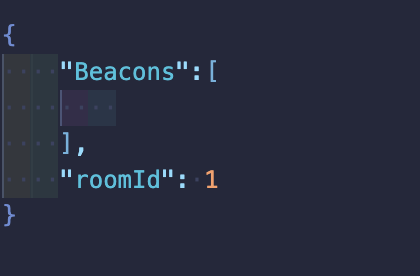
\includegraphics[width=100mm]{image/rasPost0.png}
    \caption{ビーコン情報が存在しない場合にサーバに送信するデータ}
    \label{fig:rasPost0}
  \end{center}
\end{figure}


% この手法では,メンバは常にビーコンを所持している必要がある.
% FCS1301は小型で薄いビーコンのため,財布の中や鍵のキーホルダーとして貴重品などと一緒に持ち歩ける.
% この手法では,メンバはビーコンを保持していれば一時的に部屋を出た場合にも在室判定ができ,在室者情報を記録できる.



\begin{table}[H]
  \begin{center}
    \caption{高周波 (RF) 電波を反射/吸収する物質}
    \label{tb:rf}
    \begin{tabular}{|c||c|c|c|c|c|c|c|c|c|} \hline
      障壁の種類  & 木材 & 合成物質 & ガラス & 水 & 煉瓦 & 大理石 & 土壁 & コンクリート & 金属    \\ \hline
      干渉の可能性 & 低  & 低    & 低   & 中 & 中  & 中   & 高  & 高      & 非常に高い \\ \hline
    \end{tabular}
  \end{center}
\end{table}

記録した在室者情報はWeb APIを通して利用可能であり,他のプログラムからも利用できる.
具体例として滞在ウォッチのWebサイトが挙げられる.
Webサイトを図\ref{fig:stayer}に示す.
カラムの一番左には現在の在室者の名前が表示される.これは一意な利用者の名前である.
真ん中のカラムには利用者の属性が表示される.図では研究室の名前,研究室における所属するグループの名前,現在の学年が表示されている.
右のカラムには部屋の研究室の名前と部屋名が表示される.
部屋名のみでは研究室によって同じ名前を使用している可能性があるため,研究室名も表示している.





\begin{figure}[H]
  \begin{center}
    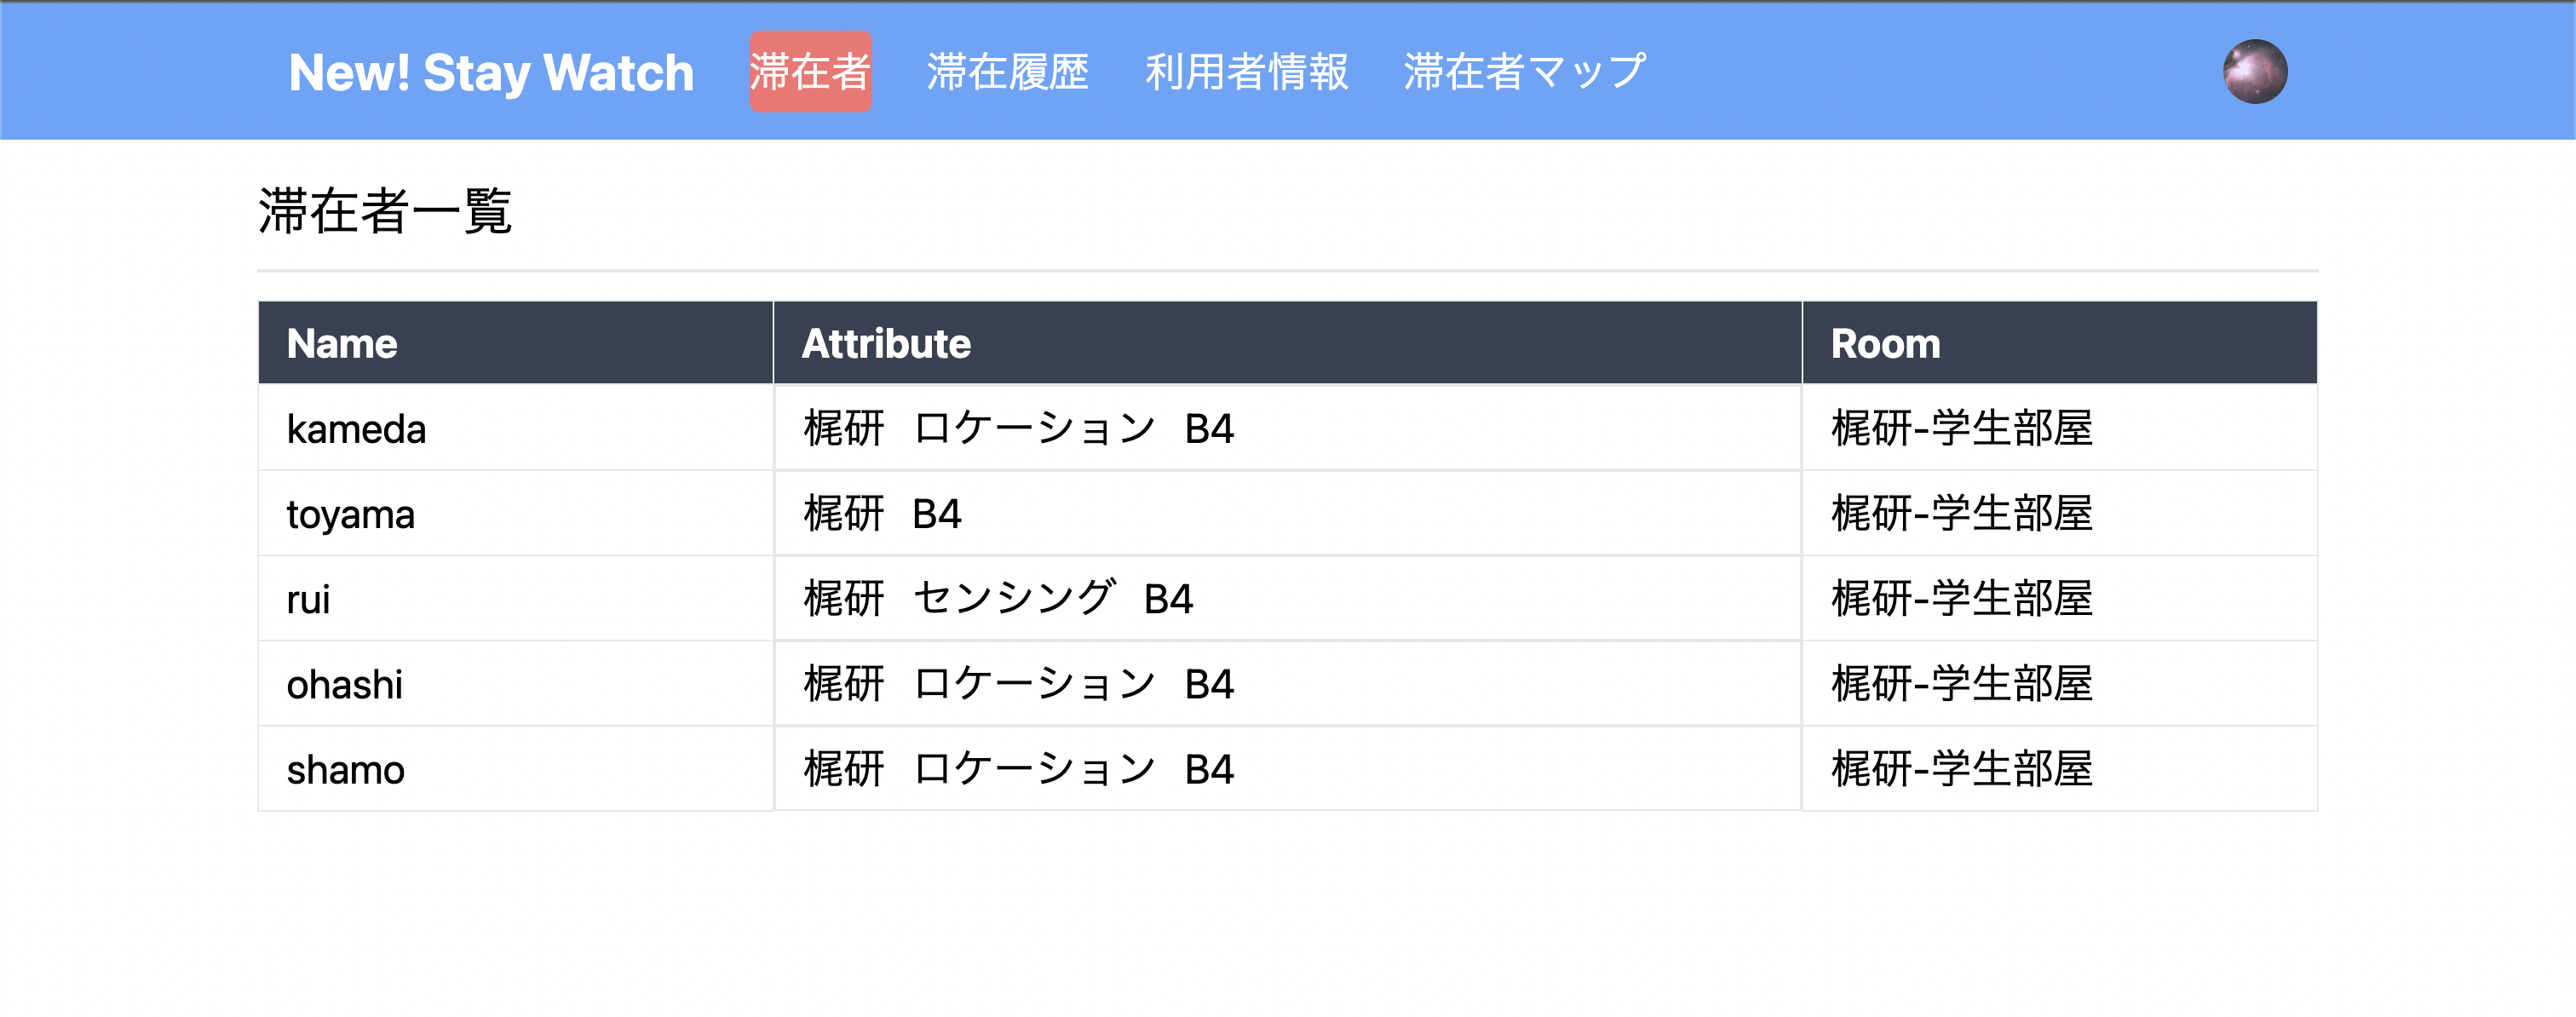
\includegraphics[width=160mm]{image/stayer.png}
    \caption{在室者の一覧画面}
    \label{fig:stayer}
  \end{center}
\end{figure}


% Web APIの利用方法は指定のURLを開くとJSON形式\cite{json}で取得できる.
% 例えば,https://kajilab.net/stay-watch/stay にアクセスすると現在の在室者情報が取得できる.
% 実際に取得したJSON形式の在室者情報を図\ref{jsonstay}に示す.
% 図\ref{jsonstay}に示すように,現在在室している人のID,名前,所属,在室している部屋を取得できる.
% この他にもhttps://kajilab.net/stay-watch/ に続けてリクエストパラメータがある.
% リクエストパラメータについて表\ref{request}に示す.

% \begin{figure}[H]
%   \begin{center}
%     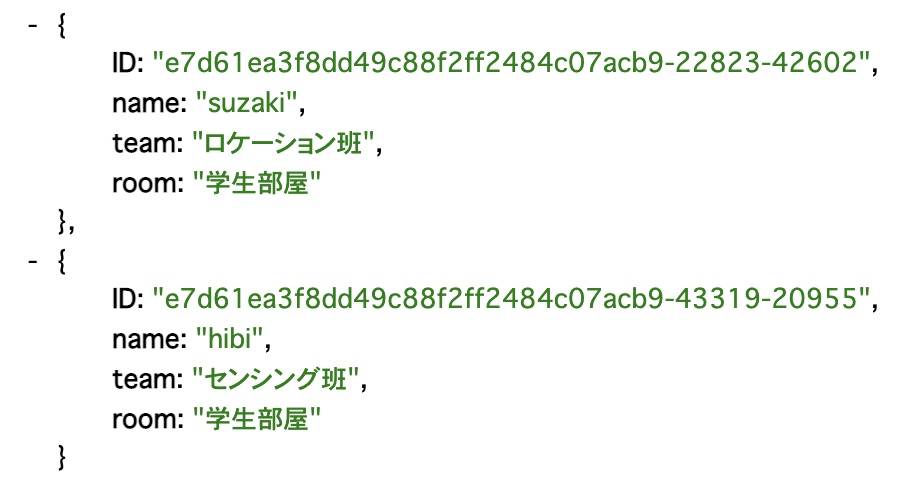
\includegraphics[width=160mm]{image/jsonstay.png}
%     \caption{JSON形式で取得した現在の在室者情報}
%     \label{jsonstay}
%   \end{center}
% \end{figure}
% \begin{table}[H]
%   \begin{center}
%     \caption{リクエストパラメータ一覧}
%     \label{request}
%     \begin{tabular}{|l|c|c|} \hline
%       パラメータ             & 値     & 説明                                       \\ \hline
%       stay                   & string & 現在の在室者を取得する                     \\ \hline
%       log                    & string & 今日の在室情報のみを取得する               \\ \hline
%       log?date1= YYYY-MM-DD
%                              & string & 過去の在室情報を取得(date1からdate2)       \\

%       \&date2=MMMM-YY-DD     &        &                                            \\\hline
%       last-time              & string & 最後に滞在を確認できた時間を取得する       \\ \hline
%       log-time               & string & 過去の累計滞在時間を取得する               \\ \hline
%       log-time?month=YYYY-MM & string & 過去の累計滞在時間を月ごとに取得する       \\ \hline
%       log-group              & stirng & その日だけのグループの滞在情報を取得する   \\ \hline
%       log-group?date1=YYYY-MM-DD
%                              & stirng & 期間を指定してグループの滞在情報を取得する \\
%       \&date2=YYYY-MM-DD     &        & (date1からdate2)                           \\\hline
%     \end{tabular}
%   \end{center}
% \end{table}